\documentclass[a4paper]{article}
% Этот шаблон документа разработан в 2014 году
% Данилом Фёдоровых (danil@fedorovykh.ru) 
% для использования в курсе 
% <<Документы и презентации в \LaTeX>>, записанном НИУ ВШЭ
% для Coursera.org: http://coursera.org/course/latex .
% Исходная версия шаблона --- 
% https://www.writelatex.com/coursera/latex/5.3

% В этом документе преамбула

\usepackage{siunitx}
%%% Работа с русским языком
%\usepackage{cmap}					% поиск в PDF
%\usepackage{mathtext} 				% русские буквы в формулах
%\usepackage[T2A]{fontenc}			% кодировка
%\usepackage[utf8]{inputenc}			% кодировка исходного текста
%\usepackage[english,russian]{babel}	% локализация и переносы
%\usepackage{indentfirst}
%\frenchspacing
%
%\renewcommand{\epsilon}{\ensuremath{\varepsilon}}
%\newcommand{\phibackup}{\ensuremath{\phi}}
%\renewcommand{\phi}{\ensuremath{\varphi}}
%\renewcommand{\varphi}{\ensuremath{\phibackup}}
%\renewcommand{\kappa}{\ensuremath{\varkappa}}
%\renewcommand{\le}{\ensuremath{\leqslant}}
%\renewcommand{\leq}{\ensuremath{\leqslant}}
%\renewcommand{\ge}{\ensuremath{\geqslant}}
%\renewcommand{\geq}{\ensuremath{\geqslant}}
%\renewcommand{\emptyset}{\varnothing}
%\renewcommand{\Im}{\operatorname{Im}}
%\renewcommand{\Re}{\operatorname{Re}}


%%% Дополнительная работа с математикой
\usepackage{amsmath,amsfonts,amssymb,amsthm,mathtools} % AMS
%\usepackage{icomma} % "Умная" запятая: $0,2$ --- число, $0, 2$ --- перечисление

%% Номера формул
%\mathtoolsset{showonlyrefs=true} % Показывать номера только у тех формул, на которые есть \eqref{} в тексте.
%\usepackage{leqno} % Нумереация формул слева

%% Свои команды
\DeclareMathOperator{\sgn}{\mathop{sgn}}
\DeclareMathOperator{\sign}{\mathop{sign}}
\DeclareMathOperator*{\res}{\mathop{res}}
\DeclareMathOperator*{\tr}{\mathop{tr}}
\DeclareMathOperator*{\rot}{\mathop{rot}}
\DeclareMathOperator*{\divop}{\mathop{div}}
\DeclareMathOperator*{\grad}{\mathop{grad}}

%% Перенос знаков в формулах (по Львовскому)
\newcommand*{\hm}[1]{#1\nobreak\discretionary{}
{\hbox{$\mathsurround=0pt #1$}}{}}

%%% Работа с картинками
\usepackage{graphicx}  % Для вставки рисунков
\graphicspath{{figures/}}  % папки с картинками
\setlength\fboxsep{3pt} % Отступ рамки \fbox{} от рисунка
\setlength\fboxrule{1pt} % Толщина линий рамки \fbox{}
\usepackage{wrapfig} % Обтекание рисунков текстом

%%% Работа с таблицами
\usepackage{array,tabularx,tabulary,booktabs} % Дополнительная работа с таблицами
\usepackage{longtable}  % Длинные таблицы
\usepackage{multirow} % Слияние строк в таблице

%%% Теоремы
\theoremstyle{plain} % Это стиль по умолчанию, его можно не переопределять.
\newtheorem{thm}{Теорема}
\newtheorem*{thm*}{Теорема}
\newtheorem{prop}{Предложение}
\newtheorem*{prop*}{Предложение}
 
\theoremstyle{definition} % "Определение"
%\newtheorem{corollary}{Следствие}[theorem]
\newtheorem{dfn}{Определение}
\newtheorem*{dfn*}{Определение}
\newtheorem{prob}{Задача}
\newtheorem*{prob*}{Задача}

 
\theoremstyle{remark} % "Примечание"
\newtheorem*{sol}{Решение}
\newtheorem*{rem}{Замечание}

%%% Программирование
\usepackage{etoolbox} % логические операторы

%%% Страница
%\usepackage{extsizes} % Возможность сделать 14-й шрифт
%\usepackage{geometry} % Простой способ задавать поля
%	\geometry{top=25mm}
%	\geometry{bottom=35mm}
%	\geometry{left=35mm}
%	\geometry{right=20mm}
 
\usepackage{fancyhdr} % Колонтитулы
%	\pagestyle{fancy}
 %	\renewcommand{\headrulewidth}{0pt}  % Толщина линейки, отчеркивающей верхний колонтитул
	%\lfoot{Нижний левый}
	%\rfoot{Нижний правый}
	%\rhead{Верхний правый}
	%\chead{Верхний в центре}
	%\lhead{Верхний левый}
	%\cfoot{Нижний в центре} % По умолчанию здесь номер страницы

\usepackage{setspace} % Интерлиньяж
%\onehalfspacing % Интерлиньяж 1.5
%\doublespacing % Интерлиньяж 2
%\singlespacing % Интерлиньяж 1

\usepackage{lastpage} % Узнать, сколько всего страниц в документе.

\usepackage{soul} % Модификаторы начертания

\usepackage{hyperref}
\usepackage[usenames,dvipsnames,svgnames,table,rgb]{xcolor}
\hypersetup{				% Гиперссылки
    unicode=true,           % русские буквы в раздела PDF
    pdftitle={Заголовок},   % Заголовок
    pdfauthor={Автор},      % Автор
    pdfsubject={Тема},      % Тема
    pdfcreator={Создатель}, % Создатель
    pdfproducer={Производитель}, % Производитель
    pdfkeywords={keyword1} {key2} {key3}, % Ключевые слова
%    colorlinks=true,       	% false: ссылки в рамках; true: цветные ссылки
    %linkcolor=red,          % внутренние ссылки
    %citecolor=black,        % на библиографию
    %filecolor=magenta,      % на файлы
    %urlcolor=cyan           % на URL
}

\usepackage{csquotes} % Еще инструменты для ссылок

%\usepackage[style=apa,maxcitenames=2,backend=biber,sorting=nty]{biblatex}

\usepackage{multicol} % Несколько колонок

\usepackage{tikz} % Работа с графикой
\usepackage{pgfplots}
\usepackage{pgfplotstable}
%\usepackage{coloremoji}
\usepackage{floatrow}
\usepackage{subcaption}
\graphicspath{{figures/}}

\renewcommand\thesubfigure{\asbuk{subfigure}}
%\addbibresource{master.bib}

\usepackage{import}
\usepackage{pdfpages}
\usepackage{transparent}
\usepackage{xcolor}
\usepackage{xifthen}

\newcommand{\incfig}[2][1]{%
    \def\svgwidth{#1\columnwidth}
    \import{./figures/}{#2.pdf_tex}
}
%\usepackage{titlesec}
%\titleformat{\section}{\normalfont\Large\bfseries}{}{0pt}{}
%----------------------STANDART:
%\titleformat{\chapter}[display]
%  {\normalfont\huge\bfseries}{\chaptertitlename\ \thechapter}{20pt}{\Huge}
%\titleformat{\section}{\normalfont\Large\bfseries}{\thesection}{1em}{}
%\titleformat{\subsection}
%  {\normalfont\large\bfseries}{\thesubsection}{1em}{}
%\titleformat{\subsubsection}
%  {\normalfont\normalsize\bfseries}{\thesubsubsection}{1em}{}
%\titleformat{\paragraph}[runin]
%  {\normalfont\normalsize\bfseries}{\theparagraph}{1em}{}
%\titleformat{\subparagraph}[runin]
%  {\normalfont\normalsize\bfseries}{\thesubparagraph}{1em}{}

\pdfsuppresswarningpagegroup=1
\pgfplotsset{compat=1.16}



%\setcounter{tocdepth}{1} % only parts,chapters,sections
%\titleformat{\subsection}{\normalfont\large\bfseries}{}{0em}{}
%\titleformat{\subsubsection}{\normalfont\normalsize\bfseries}{}{0em}{}

%\newcommand{\textover}[2]{\stackrel{\mathclap{\normalfont\mbox{#2}}}{#1}}

\author{Yaroslav Drachov\\
Moscow Institute of Physics and Technology}
%\author{Драчов Ярослав\\
%Факультет общей и прикладной физики МФТИ}
\newcommand{\veq}{\mathrel{\rotatebox{90}{$=$}}}
%\newcommand{\teto}[1]{\stackrel{\mathclap{\normalfont\tiny\mbox{#1}}}{\to}}
%\renewcommand{\thesubsection}{\arabic{subsection}}

%%\setcounter{secnumdepth}{0}

\definecolor{tabblue}{RGB}{30, 119, 180}
\definecolor{taborange}{RGB}{255, 127, 15}
\definecolor{tabgreen}{RGB}{45, 160, 43}
\definecolor{tabred}{RGB}{214, 38, 40}
\definecolor{tabpurple}{RGB}{148, 103, 189}
\definecolor{tabbrown}{RGB}{140, 86, 76}
\definecolor{tabpink}{RGB}{227, 119, 193}
\definecolor{tabgray}{RGB}{127, 127, 127}
\definecolor{tabolive}{RGB}{188, 189, 33}
\definecolor{tabcyan}{RGB}{22, 190, 207}
\pgfplotscreateplotcyclelist{colorbrewer-tab}{
{tabblue},
{taborange},
{tabgreen},
{tabred},
{tabpurple},
{tabbrown},
{tabpink},
{tabgray},
{tabolive},
{tabcyan},
}
\usepackage{csvsimple}
\usepackage{extarrows}
%\renewcommand{\labelenumii}{\asbuk{enumii})}
%\renewcommand{\labelenumiv}{\Asbuk{enumiv}}
%\newcommand{\prob}[1]{\subsubsection*{#1}}
\sisetup{output-decimal-marker = {,},separate-uncertainty = true,exponent-product = \cdot}

\usepackage{braket}
\usepackage{enumerate}
\usepackage{chngcntr}
%\counterwithin*{equation}{problem}
%\usepackage{bbold}

\newtheoremstyle{hiProb}% ⟨name ⟩ 
{3pt}% ⟨Space above ⟩1 
{3pt}% ⟨Space below ⟩1
{}% ⟨Body font ⟩
{}% ⟨Indent amount ⟩2
{\bfseries}% ⟨Theorem head font⟩
{.}% ⟨Punctuation after theorem head ⟩
{.5em}% ⟨Space after theorem head ⟩3
%{\thmname{#1} \thmnote{#3}}% ⟨Theorem head spec (can be left empty, meaning ‘normal’)⟩
{\thmnote{#3}}% ⟨Theorem head spec (can be left empty, meaning ‘normal’)⟩
\theoremstyle{hiProb} % "Определение"
%\newtheorem{hiProb}{Задача}
\newtheorem{hiProb}{}
%\usepackage{mmacells}
\newcommand{\textover}[2]{\stackrel{\mathclap{\normalfont\scriptsize\mbox{#2}}}{#1}}
\usepackage{units}
\usepackage[math]{cellspace}%
\setlength\cellspacetoplimit{2pt}
\setlength\cellspacebottomlimit{2pt}

\DeclareMathAlphabet{\mathbbold}{U}{bbold}{m}{n}

\newcommand{\normord}[1]{:\mathrel{#1}:}

\title{Лабораторная работа №8.1\\
Определение постоянных Стефана-Больцмана и Планка из
анализа теплового излучения нагретого тела}
\begin{document}
	\maketitle
\section{Изучение работы оптического пирометра}
Значение яркостной температуры модели АЧТ по шкале пирометра
$T_{\text{ярк}}=\num{1113(1)} ^\circ \text{С}$. Значение температуры
модели АЧТ, измеренное при помощи хромель-алюмелевой термопары
\[T_{\text{термопары}}=\frac{\num{48.0(10)} \text{ мВ}}{\num{41.0
(10)}\text{ мкВ}/ ^\circ \text{С}}=\num{117(4)e1} ^\circ\text{С}.\]
Значения температуры, полученные обоими способами, мало отличаются друг от друга (не более 5\%) и, следовательно, оптический
пирометр работает исправно.
\section{Измерение яркостной температуры накалённых тел}
Измерения яркостной температуры поверхности трубки и каждого из
колец приведены в табл.~\ref{tab:1}
\begin{table}[htpb]
	\centering
	\caption{Яркостная температура трубки и колец}
	\label{tab:1}
	\begin{tabular}{|c|c|}\hline
	Трубка & 887 $^\circ$C \\ \hline
	1, 3 кольца & 797 $^\circ$С \\ \hline
	2, 4 кольца & 756 $^\circ$С \\ \hline
	\end{tabular}
\end{table}
Различие яркостных температур колец при их одинаковой термодинамической
температуре объясняется тем, что эти две величины связаны, в том
числе, через спектральный коэффициент поглощения, который у
разных материалов различный.
\section{Проверка закона Стефана-Больцмана}
Экспериментальные данные измерений температуры $T_\text{ярк}$, величины
тока $I$ и падения напряжения на нити лампы $V$ представлены
в табл.~\ref{tab:2}.
	\begin{table}[htpb]
		\centering
		\caption{Экспериментальные данные}
		\label{tab:2}
		\csvreader[tabular=|c|c|c|,
		table head={\hline $T_\text{ярк},^\circ$С & $I$, А &
		$V$, В\\\hline},
		late after line=\\\hline, head to column names]
		{data.csv}{}
			{\Texp & \num{\Iexp} & \num{\Vexp}}
	\end{table}
Зависимость $T=f(T_\text{ярк})$, представленную на графике в лабораторном
практикуме по общей физике (рис.~\ref{fig:1}) \begin{figure}[htpb]
	\centering
	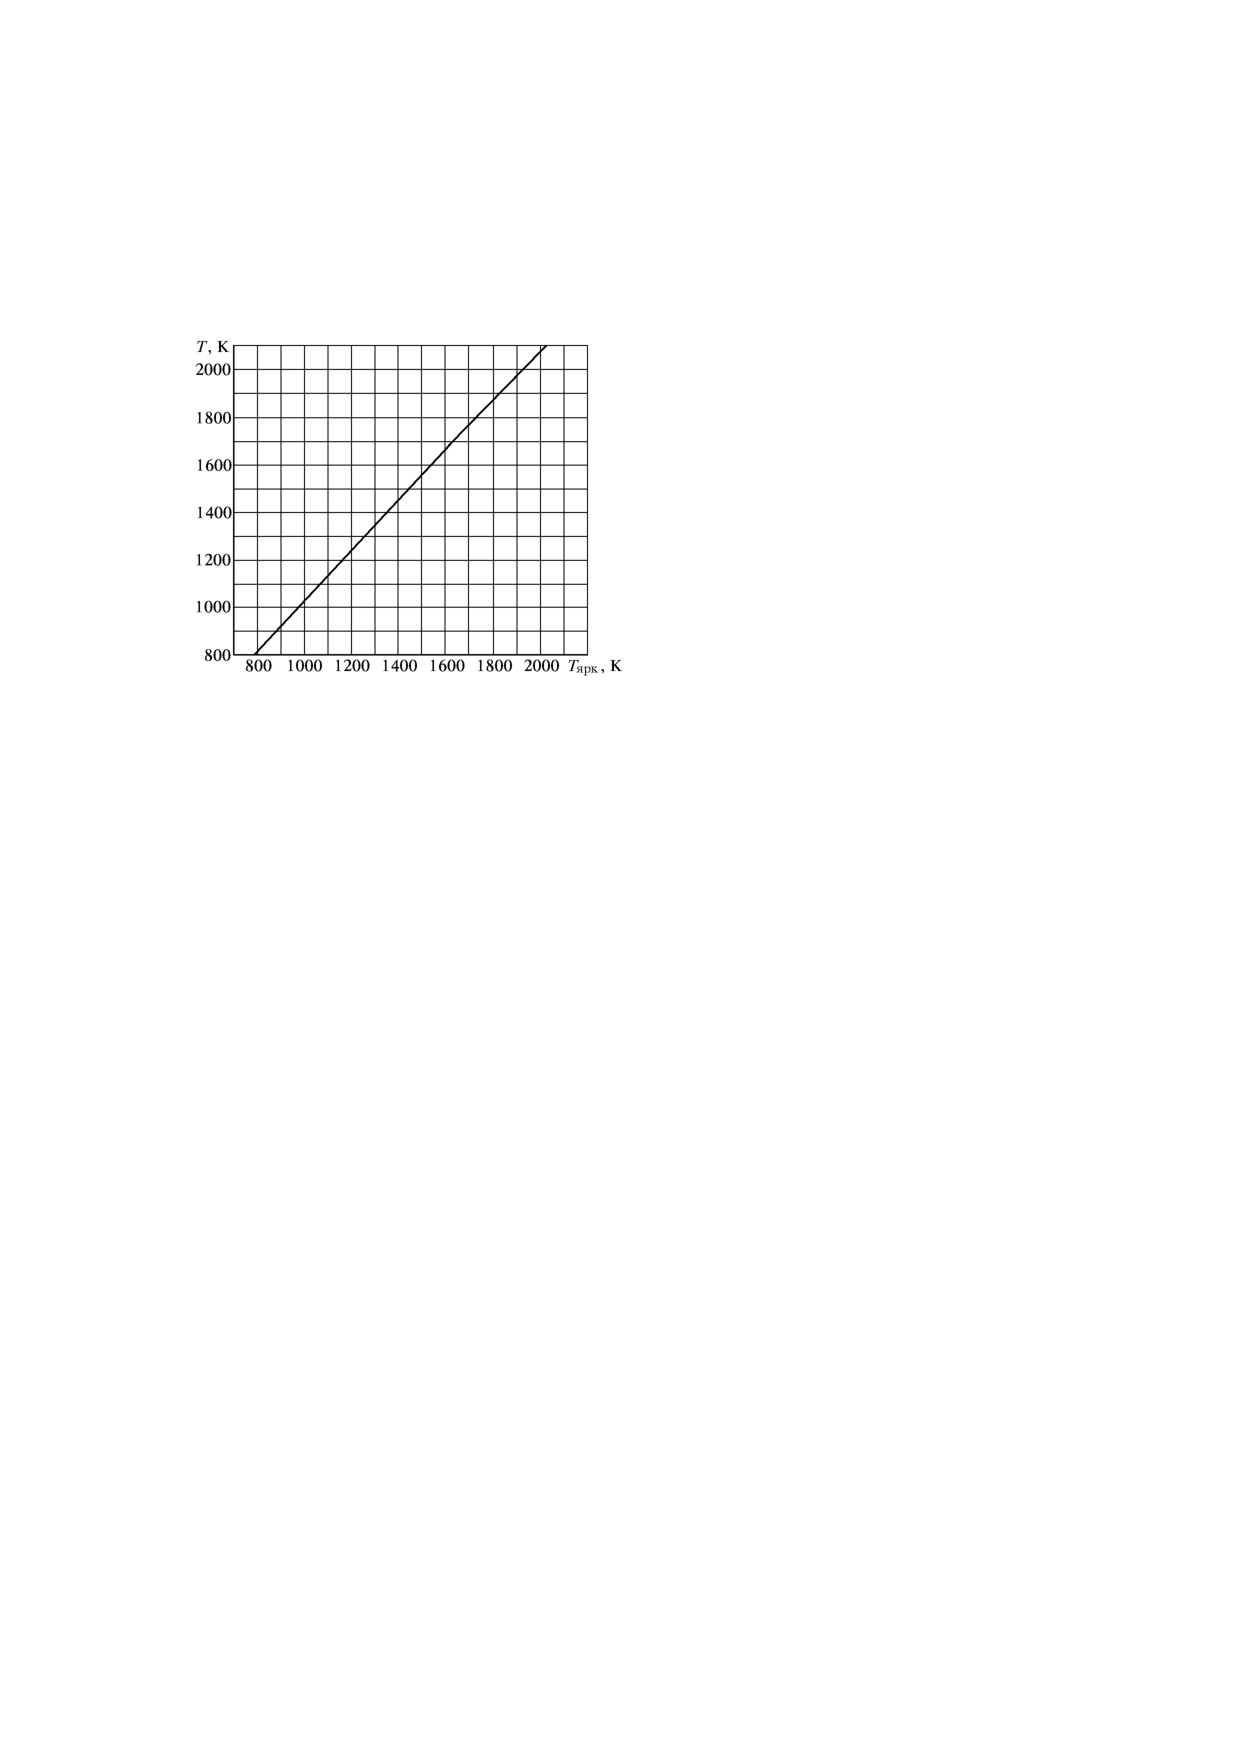
\includegraphics[width=0.8\textwidth]{1}
	\caption{График зависимости $T=f(T_\text{ярк})$ для
	вольфрама}
	\label{fig:1}
\end{figure}
можно с определённой
точностью считать линейной вида $T=-66,7+ 1,083\cdot T_\text{ярк}$. Для каждого значения термодинамической температуры
вычислим мощность, потребляемую нитью лампы по формуле
$W=UI$, полученные данные представлены в табл.~\ref{tab:3}.
	\begin{table}[htpb]
		\centering
		\caption{Зависимость мощности, потребляемой
		нитью лампы, $W$ от термодинамической температуры $T$}
		\label{tab:3}
		\csvreader[tabular=|c|c|,
		table head={\hline $T,^\circ$С & $W$, Вт \\\hline},
		late after line=\\\hline, head to column names]
		{datasethi.csv}{}
		{\num{\Texphi} & \num{\Wexp}}
	\end{table}
	График зависимости $W=f_2(T)$ представлен на  рис.~\ref{fig:2}.
\begin{figure}[htpb]
	\centering
	\begin{tikzpicture} 
		\begin{axis}
			[cycle list name=colorbrewer-tab,
			minor x tick num=0,
			minor y tick num=1,
			xlabel={$T,^\circ$C},
			ylabel={$W$, Вт},
			grid=both,]
			\addplot+ [
			only marks, error bars/.cd,
			x dir=both, x explicit,
			y dir=both, y explicit,
			] table [x=TexpAbs, x error=TexpErr, y=WexpAbs, y error=WexpErr,
			col sep= comma]{dataerr.csv};
			%\addplot+ [domain=-0:0.4,samples=201] {
			%0.5 - x};
		\end{axis}
	\end{tikzpicture}
	\caption{Зависимость $W=f_2(T)$}
	\label{fig:2}
\end{figure}
Для проверки закона Стефана-Больцмана построим в логарифмическом
масштабе график зависимости $W=\epsilon_T B T^n$ (рис.~\ref{fig:3}), т.\:е.
функцию
\[
	\ln W=\ln(\epsilon_T B)+n \ln T
.\]
\begin{figure}[htpb]
	\centering
	\begin{tikzpicture} 
		\begin{loglogaxis}
			[cycle list name=colorbrewer-tab,
			%minor x tick num=1,
			%minor y tick num=1,
			xlabel={$T$, К},
			ylabel={$W$, Вт},
			xticklabel style={/pgf/number format/.cd, use comma},
			yticklabel style={/pgf/number format/.cd, use comma},
			grid=both,
			max space between ticks=20,
			]
			\addplot+ [
			only marks, error bars/.cd,
			x dir=both, x explicit,
			y dir=both, y explicit,
			] table [x=TexpAbs, x error=TexpErr, y=WexpAbs, y error=WexpErr,
			col sep= comma]{dataerr3.csv};
			\addplot+ [domain=1191.8:2264.0,samples=201,color=tabblue] {
			1.14e-11 *x^3.92};
		\end{loglogaxis}
	\end{tikzpicture}
	\caption{График зависимости $W=\epsilon_T B T^n$ в 
	логарифмическом масштабе}
	\label{fig:3}
\end{figure}Из данной зависимости получаем $n=3,92\pm 0,14$, что в пределах
погрешности совпадает с числом 4.
Найдём величину постоянной Стефана-Больцмана по формуле
\[
\sigma= \frac{W}{\epsilon_T S T^4}
\]
для каждого измеренного значения $T$, превыщающего 1700 К.
Результаты данных вычислений приведены в табл.~\ref{tab:4}.
	\begin{table}[htpb]
		\centering
		\caption{}
		\label{tab:4}
		\csvreader[tabular=|c|c|,
		table head={\hline $T$, К & $\sigma,\, 10^{-12}\text{Вт}\cdot\text{см}^{-2}\cdot \text{К}^{-4}$ \\\hline},
		late after line=\\\hline, head to column names]
		{data4.csv}{}
		{\num{\texp} & \num{\sigmahi}}
	\end{table}
	Среднее значение по серии измерений \[\sigma=(5,21\pm 0,18)\cdot 10^{-12}\frac{\text{Вт}}{\text{см}^{-2}\cdot \text{К}^{-4}}.\]
По формуле
\[
	h= \sqrt[3]{\frac{2 \pi^5 k_\text{Б}^4}{15c^2\sigma}} 
\]
определим значение постоянной Планка \[h=(6,81\pm 0,08)\cdot
10^{-27} \text{ эрг}\cdot\text{с}.\]

Полученные значения $\sigma$ и $h$ почти сходятся с табличными.
\section{Измерение <<яркостной температуры>> неоновой
лампочки}
Измеренная пирометром <<яркостная температура>> неоновой лампочки
равна $T_\text{ярк}=875^\circ$С, однако дотронувшись до лампочки
рукой, можно отметить, что термодинамическая температура
лампочки не соответствует измеренной <<яркостной температуре>>
нагретого тела. Это объясняется тем, что неоновая лампочка
впринципе не является моделью абсолютно чёрного или серого тела, её
излучение носит совершенно другую природу (переход электронов
между энергетическими уровнями). То, что её свет имеет такой
же цвет, что и нагретое АЧТ --- совпадение.
\end{document}
